\documentclass{beamer}
\usepackage{graphicx}
\usepackage{multirow}
\usepackage[utf8]{inputenc}
\usepackage[UKenglish]{babel}
\usepackage[UKenglish]{isodate}
\usepackage[style=authoryear]{biblatex}
\usepackage{tikz}
\usepackage[clock]{ifsym}
\usepackage{adjustbox}
\usepackage{booktabs}
\usepackage{csquotes}
\usepackage{array}
\usepackage[group-separator={,}]{siunitx}
\usetikzlibrary{positioning, shapes.arrows}

\usetheme{Bergen}
%\usecolortheme{beaver}
\beamertemplatenavigationsymbolsempty
\addbibresource{../dissertation/references.bib}

\author[Paulius Dilkas]{Paulius Dilkas \inst{1} \and Ciaran McCreesh \inst{2}}
\institute[UoE]{\inst{1} University of Edinburgh, UK \and %
                      \inst{2} University of Glasgow, UK}
\title{Maximum Common Subgraph}
\subtitle{Algorithms and Algorithm Portfolios}
\date{LJMS 8}

\DeclareMathOperator{\E}{E}
\DeclareMathOperator{\nablaop}{\nabla}

\begin{document}
{
  \usebackgroundtemplate{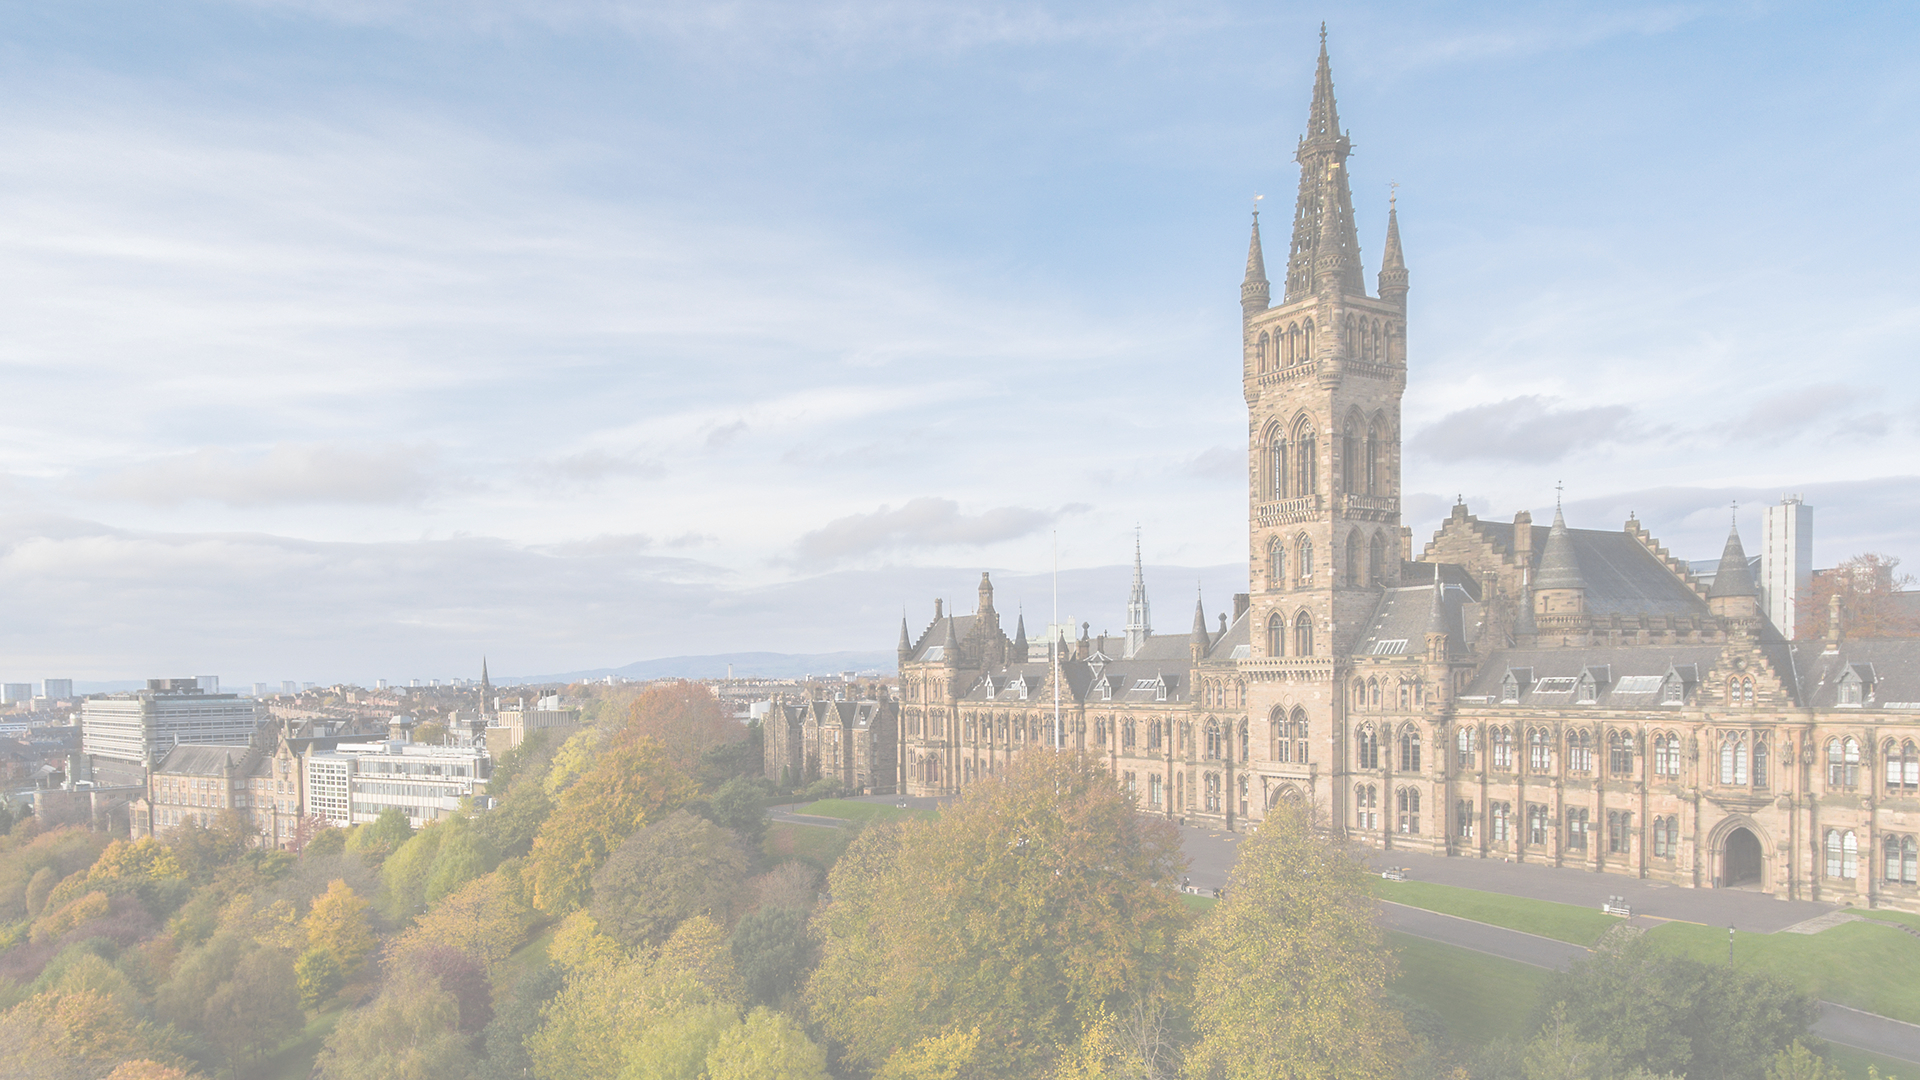
\includegraphics[trim={1cm 0 0 0},clip,height=\paperheight]{gla2.jpg}}
  \maketitle
}

{
  \usebackgroundtemplate{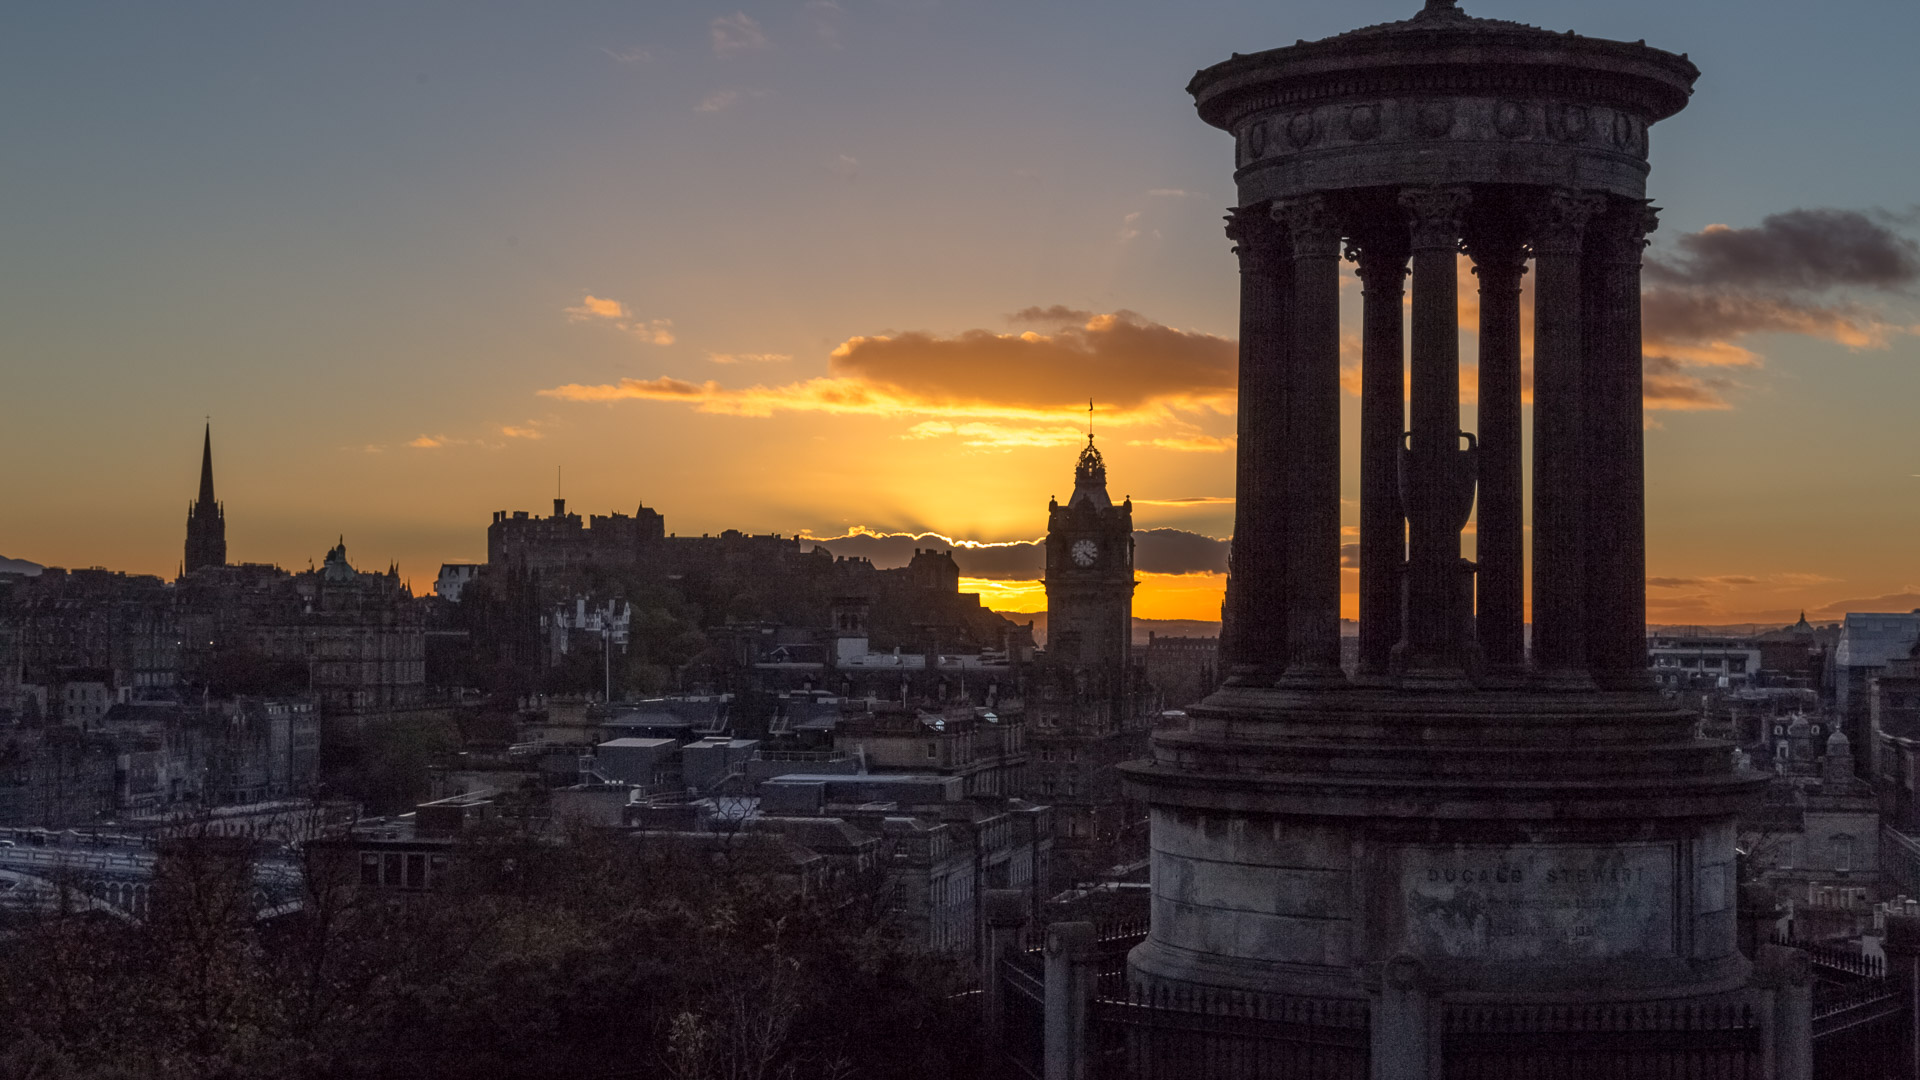
\includegraphics[trim={12cm 0 0 0},clip,height=\paperheight]{dark.jpg}}
  \begin{frame}{Outline}
    \tableofcontents
  \end{frame}
}

\section{The Problem}

\begin{frame}{Maximum Common Subgraph}
  \begin{definition}
    A \emph{maximum common (induced) subgraph} between graphs $G_1$ and
    $G_2$ is a graph $G_3 = (V_3, E_3)$ such that $G_3$ is isomorphic to induced
    subgraphs of both $G_1$ and $G_2$ with $|V_3|$ maximised.
  \end{definition}
  \begin{adjustbox}{max totalsize={0.5\textwidth}{0.5\textheight},center}
    \begin{tikzpicture}
      \begin{scope}[every node/.style={circle,draw}]
        \node (u1) [fill=lightgray,] at (0, 5) {$u_1$};
        \node (u2) at (0, 3) {$u_2$};
        \node (u3) at (0, 1) {$u_3$};
        \onslide<1>{\node (u4) at (2, 4) {$u_4$};}
        \onslide<1>{\node (u5) at (2, 2) {$u_5$};}
      \end{scope}
      \node (name1) at (1, 0) {$G_1$};
      \path (u1) [color=blue,ultra thick] edge node {} (u2);
      \onslide<1>{\path (u1) edge node {} (u4);}
      \onslide<1>{\path (u1) edge node {} (u5);}
      \onslide<1>{\path (u2) edge node {} (u4);}
      \onslide<1>{\path (u3) edge node {} (u4);}
      \onslide<1>{\path (u3) edge node {} (u5);}
      \begin{scope}[every node/.style={circle, draw},xshift=4cm]
        \node (v1) at (0, 5) {$v_1$};
        \onslide<1>{\node (v2) at (0, 3) {$v_2$};}
        \node (v3) at (0, 1) {$v_3$};
        \node (v4) [fill=lightgray] at (2, 4) {$v_4$};
        \onslide<1>{\node (v5) [fill=lightgray] at (2, 2) {$v_5$};}
      \end{scope}
      \node (name2) [xshift=4cm] at (1, 0) {$G_2$};
      \begin{scope}[color=blue,ultra thick]
        \onslide<1>{\path (v1) edge node {} (v2);}
        \path (v1) edge node {} (v4);
        \onslide<1>{\path (v2) edge node {} (v4);}
        \onslide<1>{\path (v2) edge node {} (v5);}
      \end{scope}
      \begin{scope}[color=red,thick]
        \onslide<2->{\path[->] (u1) edge [bend left=40] (v4);}
        \onslide<2->{\path[->] (u2) edge (v1);}
        \onslide<2->{\path[->] (u3) edge (v3);}
      \end{scope}
    \end{tikzpicture}
  \end{adjustbox}
\end{frame}

\section{Algorithms}

\begin{frame}{Clique Encoding}
      %\vspace{-6cm}
      \begin{adjustbox}{max totalsize={0.4\textwidth}{0.99\textheight},left}
        \begin{tikzpicture}
          \begin{scope}[every node/.style={circle,draw}]
            \node (u1) [fill=lightgray,] at (0, 5) {$u_1$};
            \node (u2) at (0, 3) {$u_2$};
            \node (u3) at (0, 1) {$u_3$};
            \node (u4) at (2, 4) {$u_4$};
            \node (u5) at (2, 2) {$u_5$};
          \end{scope}
          \path (u1) [color=blue,ultra thick] edge node {} (u2);
          \path (u1) edge node {} (u4);
          \path (u1) edge node {} (u5);
          \path (u2) edge node {} (u4);
          \path (u3) edge node {} (u4);
          \path (u3) edge node {} (u5);
          \begin{scope}[every node/.style={circle, draw},xshift=4cm]
            \node (v1) at (0, 5) {$v_1$};
            \node (v2) at (0, 3) {$v_2$};
            \node (v3) at (0, 1) {$v_3$};
            \node (v4) [fill=lightgray] at (2, 4) {$v_4$};
            \node (v5) [fill=lightgray] at (2, 2) {$v_5$};
          \end{scope}
          \begin{scope}[color=blue,ultra thick]
            \path (v1) edge node {} (v2);
            \path (v1) edge node {} (v4);
            \path (v2) edge node {} (v4);
            \path (v2) edge node {} (v5);
          \end{scope}
          \begin{scope}[color=red,thick]
            \path[->] (u1) edge [bend left=40] (v4);
            \path[->] (u2) edge [bend right=20] (v1);
            \path[->] (u3) edge [] (v3);
          \end{scope}
        \end{tikzpicture}
      \end{adjustbox}

      \vspace{-1cm}
      \begin{adjustbox}{max totalsize={0.7\textwidth}{0.99\textheight},right}
        \begin{tikzpicture}
          \begin{scope}
            \node (u1v4) [color=red,ultra thick,text=black] at (360/14 * 1:9cm) {\Huge $u_1 \mapsto v_4$};
            \node (u1v5) at (360/14 * 2:9cm) {\Huge $u_1 \mapsto v_5$};
            \node (u2v1) [color=red,ultra thick,text=black] at (360/14 * 3:9cm) {\Huge $u_2 \mapsto v_1$};
            \node (u2v2) at (360/14 * 4:9cm) {\Huge $u_2 \mapsto v_2$};
            \node (u2v3) at (360/14 * 5:9cm) {\Huge $u_2 \mapsto v_3$};
            \node (u3v1) at (360/14 * 6:9cm) {\Huge $u_3 \mapsto v_1$};
            \node (u3v2) at (360/14 * 7:9cm) {\Huge $u_3 \mapsto v_2$};
            \node (u3v3) [color=red,ultra thick,text=black] at (360/14 * 8:9cm) {\Huge $u_3 \mapsto v_3$};
            \node (u4v1) at (360/14 * 9:9cm) {\Huge $u_4 \mapsto v_1$};
            \node (u4v2) at (360/14 * 10:9cm) {\Huge $u_4 \mapsto v_2$};
            \node (u4v3) at (360/14 * 11:9cm) {\Huge $u_4 \mapsto v_3$};
            \node (u5v1) at (360/14 * 12:9cm) {\Huge $u_5 \mapsto v_1$};
            \node (u5v2) at (360/14 * 13:9cm) {\Huge $u_5 \mapsto v_2$};
            \node (u5v3) at (360/14 * 14:9cm) {\Huge $u_5 \mapsto v_3$};
          \end{scope}

          \begin{scope}[color=red,ultra thick]
            \path (u1v4) edge (u2v1) edge (u3v3);
            \path (u2v1) edge (u3v3);
          \end{scope}

          \path (u1v4) edge (u2v2);
          \path (u1v5) edge (u2v2) edge (u3v1) edge (u3v3);
          \path (u2v1) edge (u5v3);
          \path (u2v2) edge (u3v3) edge (u5v3);
          \path (u2v3) edge (u3v1) edge (u3v2) edge (u5v1) edge (u5v2);
          \path (u4v1) edge (u5v3);
          \path (u4v2) edge (u5v3);
          \path (u4v3) edge (u5v1) edge (u5v2);
        \end{tikzpicture}
      \end{adjustbox}
\end{frame}

\begin{frame}{\textsc{McSplit}: a Branch and Bound Algorithm}
  \begin{columns}
    \begin{column}{0.6\textwidth}
      \begin{adjustbox}{max totalsize={0.9\textwidth}{0.9\textheight},center}
        \begin{tikzpicture}
          \begin{scope}[every node/.style={circle,draw}]
            \node (u1) [fill=lightgray,] at (0, 5) {$u_1$};
            \node (u2) at (0, 3) {$u_2$};
            \node (u3) at (0, 1) {$u_3$};
            \node (u4) at (2, 4) {$u_4$};
            \node (u5) at (2, 2) {$u_5$};
          \end{scope}
          \node (name1) at (1, 0) {$G_1$};
          \path (u1) [color=blue,ultra thick] edge node {} (u2);
          \path (u1) edge node {} (u4);
          \path (u1) edge node {} (u5);
          \path (u2) edge node {} (u4);
          \path (u3) edge node {} (u4);
          \path (u3) edge node {} (u5);
          \begin{scope}[every node/.style={circle, draw},xshift=4cm]
            \node (v1) at (0, 5) {$v_1$};
            \node (v2) at (0, 3) {$v_2$};
            \node (v3) at (0, 1) {$v_3$};
            \node (v4) [fill=lightgray] at (2, 4) {$v_4$};
            \node (v5) [fill=lightgray] at (2, 2) {$v_5$};
          \end{scope}
          \node (name2) [xshift=4cm] at (1, 0) {$G_2$};
          \begin{scope}[color=blue,ultra thick]
            \path (v1) edge node {} (v2);
            \path (v1) edge node {} (v4);
            \path (v2) edge node {} (v4);
            \path (v2) edge node {} (v5);
          \end{scope}
          \begin{scope}[color=red,thick]
            \onslide<2->{\path[->] (u1) edge [bend left=40] (v4);}
            \onslide<8->{\path[->] (u2) edge [bend right=20] (v1);}
            \onslide<5->{\path[->] (u3) edge [] (v3);}
          \end{scope}
        \end{tikzpicture}
      \end{adjustbox}
    \end{column}

    \begin{column}{0.4\textwidth}
      \begin{overprint}
        Upper bound: \only<1-3>{$4$}\only<4>{\alert{$1+2$}}\only<5-6>{$1+2$}\only<7>{\alert{$2+1$}}\only<8->{$2+1$}

        Partial solution:

        \only<1-2>{$\{\}$}\only<3>{$\{\alert{u_1 \mapsto v_4}\}$}\only<4-5>{\{$u_1 \mapsto v_4$\}}\only<6>{$\{u_1 \mapsto v_4, \alert{u_3 \mapsto v_3}\}$}\only<7->{$\{u_1 \mapsto v_4, u_3 \mapsto v_3\}$}
      \end{overprint}
    \end{column}
  \end{columns}
        \begin{overlayarea}{\textwidth}{3cm}
          \centering
          \only<-2>{
            \begin{tabular}{c c c}
              \toprule
              Label & $G_1$ & $G_2$ \\
              \midrule
              0 & $u_2, u_3, u_4, u_5$ & $v_1, v_2, v_3$ \\
              1 & $u_1$ & $v_4, v_5$ \\
              \bottomrule
            \end{tabular}
            \begin{overprint}
              \onslide<2>{

                Decision: $u_1 \mapsto v_4$}
            \end{overprint}
          }
          \only<3>{
            \begin{tabular}{c c c}
              \toprule
              Label & $G_1$ & $G_2$ \\
              \midrule
              00 & $u_3$ & $v_3$ \\
              01 & $u_4, u_5$ & $\emptyset$ \\
              02 & $u_2$ & $v_1, v_2$ \\
              10 & $\emptyset$ & $v_5$ \\
              \bottomrule
            \end{tabular}
          }
          \only<4-5>{
            \begin{tabular}{c c c}
              \toprule
              Label & $G_1$ & $G_2$ \\
              \midrule
              00 & $u_3$ & $v_3$ \\
              01 & $u_2$ & $v_1, v_2$ \\
              \bottomrule
            \end{tabular}
            \begin{overprint}
              \onslide<5>{

                Decision: $u_3 \mapsto v_3$
              }
            \end{overprint}
          }
          \only<6>{
            \begin{tabular}{c c c}
              \toprule
              Label & $G_1$ & $G_2$ \\
              \midrule
              010 & $u_2$ & $v_1, v_2$ \\
              011 & $u_4, u_5$ & $\emptyset$ \\
              \bottomrule
            \end{tabular}
          }
          \only<7->{
            \begin{tabular}{c c c}
              \toprule
              Label & $G_1$ & $G_2$ \\
              \midrule
              010 & $u_2$ & $v_1, v_2$ \\
              \bottomrule
            \end{tabular}
            \begin{overprint}
              \onslide<8>{

                Decision: $u_2 \mapsto v_1$\\ Found a solution! \\ Backtrack to confirm optimality
              }
            \end{overprint}
          }
        \end{overlayarea}
\end{frame}

\section{Algorithm Selection}

\begin{frame}{Which Is Better?}
  \centering
  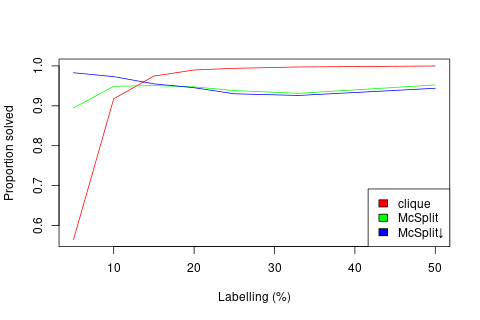
\includegraphics[width=\textwidth]{both_labels_linechart.png}
\end{frame}

\begin{frame}{(Per-Instance) Algorithm Selection}
%  \begin{definition}[\cite{DBLP:journals/ai/BischlKKLMFHHLT16}]
%    Given a set $\mathcal{I}$ of problem instances, a space of algorithms
%    $\mathcal{A}$, and a performance measure $m \colon \mathcal{I} \times
%    \mathcal{A} \to \mathbb{R}$, the \emph{algorithm selection problem} is to
%    find a mapping $s \colon \mathcal{I} \to \mathcal{A}$ that optimises
%    $\mathbb{E}[m(i, s(i))]$.
%  \end{definition}
    \centering
    \begin{tikzpicture}
      \onslide<1->{\node (graphs) at (0, 4) {$(G_1, G_2)$};}
      \onslide<2->{\node (features) at (2, 4) {$\begin{bmatrix}f_1\\ \vdots \\ f_n\end{bmatrix}$};}
      \onslide<3->{\node[draw] (ml) at (5, 4) {ML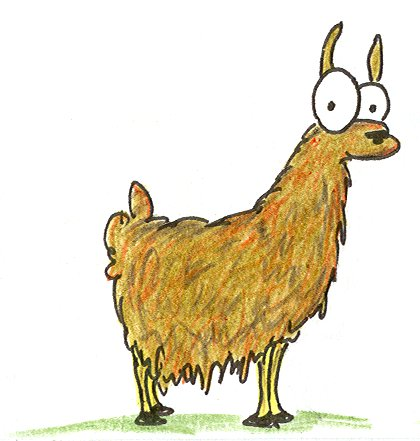
\includegraphics[scale=0.1]{llama.jpg}};}
      \onslide<4->{\node (mcsplit) at (2, 2) {\textsc{McSplit}};}
      \onslide<4->{\node (mcsplitdown) at (4, 2) {$\textsc{McSplit}{\downarrow}$};}
      \onslide<4->{\node (clique) at (6, 2) {clique};}
      \onslide<4->{\node (kdown) at (8, 2) {$k{\downarrow}$};}
      \onslide<6->{\node (answer) at (4, 0) {answer};}
      \path[->]<2-> (graphs) edge node[above] {\VarClock} (features);
      \path[->]<3-> (features) edge (ml);
      \path[->]<4-> (ml) edge (mcsplit);
      \only<1-4>{\tikzset{properties/.style={}}}
      \only<5->{\tikzset{properties/.style={ultra thick}}}
      \draw<4-> [->] (ml) edge[properties] (mcsplitdown);
      \path[->]<4-> (ml) edge (clique);
      \path[->]<4-> (ml) edge (kdown);
      \path[->]<6-> (mcsplitdown) edge node[right] {\VarClock} (answer);
      \path[->]<6-> (graphs) edge [bend right=50] (4, 1);
    \end{tikzpicture}
\end{frame}

%\begin{frame}{Features (34 in total)}
%  \begin{enumerate}
%  \item number of vertices
%  \item number of edges
%  \item mean/max degree
%  \item density
%  \item mean/max distance between pairs of vertices
%  \item number of loops
%  \item proportion of vertex pairs with distance $\ge$ 2, 3, 4
%  \item connectedness
%    \pause
%  \item standard deviation of degrees
%  \item labelling percentage
%    \pause
%  \item ratios of features 1--5
%  \end{enumerate}
%\end{frame}

\section{Results \& Observations}

\begin{frame}{Overall Performance}
  \begin{figure}
    \centering
    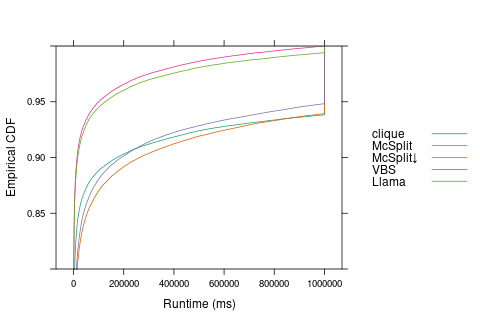
\includegraphics[width=0.9\textwidth]{ecdf_both_labels_llama.png}
  \end{figure}
\end{frame}

\begin{frame}{Observations}
  \begin{itemize}
  \item Most important features:
    \begin{itemize}
    \item labelling percentage
    \item standard deviation of degrees (for both graphs)
    \end{itemize}
  \item Looking at a single feature is not enough
%  \item $k{\downarrow}$ is no longer competitive
%  \item Unclear when \textsc{McSplit} outperforms $\textsc{McSplit}{\downarrow}$
%    \pause
%  \item No work has ben done on non-uniform distributions of labels
  \end{itemize}
  \pause
  \vfill
  \centering
  \large
  \emph{Thank You!}
\end{frame}

\end{document}
